\chapter{Metodoloxía e planificación}
\label{chap:metodoloxia}

Para realizar o traballo decidiuse seguir unha metodoloxía áxil e iterativa, ao ser un número reducido de desenvolvedores e clientes non se precisa unha estrutura xerárquica, e todas as partes poden manterse actualizadas do desenvolvemento do proxecto con facilidade. Esta metodoloxía consiste nun proceso iterativo, onde todos os interesados no desenvolvemento poden manterse ao día sobre os problemas e modificacións que van xurdindo.

\section{Funcionamento de SCRUM}

Como metodoloxía específica escolleuse SCRUM, pola súa familiaridade e popularidade. A metodoloxía SCRUM\cite{scrum} baséase nunha serie de fases («\textit{sprints}»), definidas no tempo, continuas e completas. Cada fase ten as seguintes partes:

\begin{description}
	\item[Planificación] Cada fase comezan coa súa planificación. É aquí onde se definiran os obxectivos da fase, e decidirase como realizar o traballo preciso
	\item[Reunión diaria] Diariamente os desenvolvedores reuniranse para revisar a planificación das fases, co obxectivo de atopar e arranxar calquera desviación que poida desbaratar a fase. Deberán revisar o traballo realizado dende a última reunión e planificar o traballo a realizar para a seguinte reunión
	\item[Revisión] O equipo deberá presentar unha revisión do traballo realizado na fase. Isto permitirá realizar cambios para futuras fases
	\item[Retrospectiva] Tras a revisión, pero de xeito separado, o equipo deberá realizar unha revisión centrada no proceso da fase, de xeito que se identifiquen que bloqueos existiron, como se resolveron e o seu impacto
\end{description}

\newpage

Para xestionar os obxectivos do proxecto, SCRUM prescribe a creación de tres listaxes:

\begin{enumerate}
	\item Do produto, centrado na mellora do produto no seu conxunto
	\item Da fase, un subconxunto da listaxe do produto no cal vaise traballar nesta fase. Representa un plan, que indica o obxectivo da fase e como acadalo
	\item Do incremento, pasos concretos e funcionais que permiten acadar o obxectivo do produto. Pode haber varios incrementos por fase
\end{enumerate}

Os resultados denomínanse «artefactos», e, dependendo da listaxe, poden denominarse obxectivo do produto («\textit{Project Goal}»), da fase («\textit{Sprint Goal}»); ou unha descrición de obxectivo cumprido («\textit{Definition of Done}») no caso dos incrementos. Cada obxectivo representa o punto final de cadanseu ámbito.

Dentro do equipo de SCRUM defínense varios roles:

\begin{itemize}
	\item Desenvolvedores, que son as persoas que acadan os obxectivos dos incrementos, seguindo as directrices das fases, produtos e incrementos
	\item Dono do produto, encargado de controlar os obxectivos do produto e asegurarse de que o equipo céntrase na creación de valor para o produto
	\item Xefe de SCRUM, que xestiona o proceso de SCRUM dende o punto de vista procesual e persoal, axudando ao resto de compoñentes do equipo segundo precisen.
\end{itemize}

Á hora de aplicar a metodoloxía anterior realizáronse certas modificacións para adaptalas ás particularidades dun desenvolvedor, o alumno, facendo os co-directores do proxecto de donos do produto.

As reunións realizáronse de dous xeitos. Por unha banda, e por mor das diferenzas de horario, a meirande parte das reunións foron asíncronas, mediante a plataforma de Teams. O resto foron reunións telemáticas, tamén mediante a plataforma de Teams, menos frecuentes pero de maior duración. Nestas últimas reunións realizouse unha demostración completa do funcionamento da aplicación. 

\section{Planificación}

A organización das distintas tarefas (indicadas na figura \ref{fig:gantt}) corresponde a dúas clasificacións: temática e modular.

\newpage

A clasificación temática presenta tres elementos:

\begin{enumerate}
	\item Modelos
	\item Compoñentes
	\item Usuarios
\end{enumerate}

Cada un destes elementos precisa dunha tarefa de deseño, unha tarefa de implantación e integración da API REST, e da creación da interface web correspondente. A clasificación modular corresponde ás dúas partes do sistema: cliente e servidor. Dentro da tarefa de implantación realizouse todo o traballo de programación, xestión das entidades na base de datos e conexión coa API REST, incluíndo serialización, deserialización e excepcións.

A parte do servidor inclúe o deseño e implantación da API REST, e a parte de cliente inclúe o deseño e creación da interface web.

\vspace*{5em}
\begin{figure}[htbp]
	\hspace*{-3cm}
	\centering
	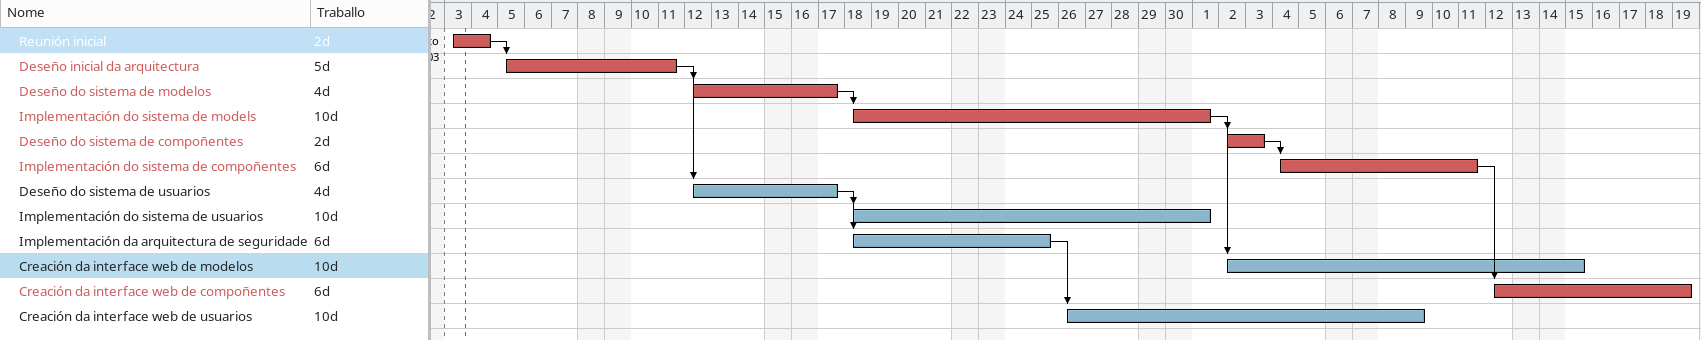
\includegraphics[width=\textwidth,width=50em]{imaxes/gantt.png}
	\caption{Diagrama de Gantt das fases do proxecto}
	\label{fig:gantt}
\end{figure}
\vspace*{5em}

Dentro do esquema de SPRINT definíronse 3 fases: modelo, compoñentes e usuarios. Dentro de cada fase incluíronse como incrementos as tarefas indicadas anteriormente.

\section{Orzamento}

A previsión do orzamento que pode precisar a realización dun proxecto depende de moitos factores únicos para cada empresa. Aquí preséntase unha posible aproximación, pensando no ambiente dunha empresa pequena. Hai dúas clases de custos: periódicos e únicos. Os custos periódicos son aqueles que se repiten cada certo tempo. Dentro deste ámbito incluiríanse os salarios dos traballadores ou as licenzas, se as houber. Os únicos corresponden á adquisición do material que precisa cada traballador, e ocorren ao inicio do proxecto.

Inda que o máis probable é que o persoal xa dispoña do material que precisa doutros proxectos, inclúese no cálculo. Para os ordenadores engadiuse un orzamento de 1000 € por desenvolvedor, e o IDE representa un custo de 724,79€ por desenvolvedor (para un ano). Isto representa 1724,79€ por desenvolvedor, e $ 10 348,74€ $.

O tamaño do equipo calcúlase en seis persoas como un tamaño óptimo\cite{chaosmanifesto}. Considerarase un salario medio anual de $ 36 000€ $\cite{ccii}\cite{confidencial}\cite{ine}. A duración dun proxecto de \textit{software} non é sinxelo de calcular, pero para este, considerando o tempo da realización deste traballo de fin de grao, escolléronse 3 meses para esta versión inicial. Isto daría un custo en salarios de $ 36000 ~ \sfrac{\text{€}}{\text{persoa} \cdot \text{ano}} \cdot 6 ~ \text{persoas} \cdot \frac{3 ~ \text{meses}}{12 ~ \tfrac{\text{meses}}{\text{ano}}} = 54000 € $ para os tres meses de desenvolvemento.

Isto representa un custo total de $ 64 348,74€ $